\documentclass[11pt,a4paper]{article}
\usepackage[utf8]{inputenc}
\usepackage[T1]{fontenc}
\usepackage{polski}
\usepackage{lmodern}
\usepackage[a4paper,margin=2cm]{geometry}
\usepackage{amsmath,amssymb}
\usepackage{graphicx}
\usepackage{booktabs,array}
\usepackage{caption}
\usepackage{microtype}
\usepackage{xcolor}
\usepackage{enumitem}
\usepackage[most]{tcolorbox}
\usepackage[colorlinks=true,linkcolor=blue,urlcolor=blue]{hyperref}
\emergencystretch=3em
\captionsetup{font=small,labelfont=bf}
\setlength{\parskip}{4pt}
\setlength{\parindent}{0pt}
\setlist{itemsep=2pt,topsep=2pt}
% generated by analysis.py - do not edit
\newcommand{\NCzero}{35.0}
\newcommand{\NDNazero}{1426}
\newcommand{\NDNazeroErr}{58}
\newcommand{\NEKnowles}{-0.319}
\newcommand{\NFpval}{0.00}
\newcommand{\NFpvalOnek}{0.009}
\newcommand{\NFstat}{9.41}
\newcommand{\NFstatOnek}{2.62}
\newcommand{\NGcalAtCzero}{-52.13}
\newcommand{\NGfromKzero}{-52.77}
\newcommand{\NISEglycerol}{6}
\newcommand{\NKzero}{1.76}
\newcommand{\NMUXKCL}{0.035}
\newcommand{\NPKnowles}{+0.396}
\newcommand{\NSKhighc}{1.14}
\newcommand{\NSKlocal}{3.47}
\newcommand{\NSKlocalErr}{0.10}
\newcommand{\NSKmodel}{2.95}
\newcommand{\NSKmodelErr}{0.05}
\newcommand{\NSdosyA}{+0.188}
\newcommand{\NSdosyB}{+0.098}
\newcommand{\NSdosyC}{+0.061}
\newcommand{\Natfourzeroa}{+11.3}
\newcommand{\Natfourzerob}{+7.7}
\newcommand{\Natfourzeroc}{+3.7}
\newcommand{\Natfourzerodone}{+2.3}
\newcommand{\Natfourzerodtwo}{+1.6}
\newcommand{\Natfourzeroe}{-4.2}
\newcommand{\NbOneCV}{19}
\newcommand{\NbOneCVOnek}{10}
\newcommand{\NbOneChi}{3.3}
\newcommand{\NbOneMean}{-0.234}
\newcommand{\NbOneMeanErr}{0.015}
\newcommand{\NbTwoCV}{5}
\newcommand{\NbTwoChi}{0.2}
\newcommand{\NbTwoMean}{+21.3}
\newcommand{\NbTwoMeanErr}{1.2}
\newcommand{\NbnCodeEG}{0.43}
\newcommand{\NbnCodeEGErr}{0.07}
\newcommand{\NbnCodePEGtwo}{0.80}
\newcommand{\NbnCodePEGtwoErr}{0.05}
\newcommand{\NbnSelfEG}{-0.034}
\newcommand{\NbnSelfEGErr}{0.154}
\newcommand{\NbnSelfPEGtwo}{0.034}
\newcommand{\NbnSelfPEGtwoErr}{0.121}
\newcommand{\NbnSelfQuadEG}{-0.066}
\newcommand{\NbnSelfQuadPEGtwo}{-0.002}
\newcommand{\NbnUpperEG}{0.27}
\newcommand{\NbnUpperPEGtwo}{0.28}
\newcommand{\NbroSone}{-0.916}
\newcommand{\NbroSoneErr}{0.225}
\newcommand{\NbroStwo}{+0.100}
\newcommand{\NbroStwoErr}{0.007}
\newcommand{\NbroSixSone}{-0.260}
\newcommand{\NbroSixSoneErr}{0.021}
\newcommand{\NbroSixStwo}{+0.185}
\newcommand{\NbroSixStwoErr}{0.021}
\newcommand{\NbroXsMax}{1.3}
\newcommand{\NbroXsMin}{-1.6}
\newcommand{\NcEGforty}{6.87}
\newcommand{\NcEqEG}{5.5}
\newcommand{\NchiFreeTot}{66}
\newcommand{\NchiJointRed}{26.5}
\newcommand{\NchiQuadTot}{407}
\newcommand{\NchiSepRed}{10.0}
\newcommand{\NchiSixTot}{435}
\newcommand{\NcollconstAllAlpha}{-0.95}
\newcommand{\NcollconstAllRtwo}{0.87}
\newcommand{\NcollconstPEGAlpha}{-0.94}
\newcommand{\NcollconstPEGRtwo}{0.86}
\newcommand{\NcollrealAlpha}{-0.75}
\newcommand{\NcollrealRtwo}{0.90}
\newcommand{\NcurvObsSigma}{14.5}
\newcommand{\Ncurva}{-35.4}
\newcommand{\Ncurvb}{-32.0}
\newcommand{\Ncurvc}{-15.7}
\newcommand{\Ncurvobs}{+93.2}
\newcommand{\NddGEGforty}{14.7}
\newcommand{\NddGEGfortyErr}{0.5}
\newcommand{\NddGobsFortyPEGthirtyfive}{-0.3}
\newcommand{\NegExplCode}{5.4}
\newcommand{\NegExplFracCode}{37}
\newcommand{\NegExplFracKappa}{20}
\newcommand{\NegExplFracUpper}{28}
\newcommand{\NegExplKappa}{2.9}
\newcommand{\NegExplUpper}{4.1}
\newcommand{\NfracMaxa}{77}
\newcommand{\NfracMaxb}{45}
\newcommand{\NfracMaxc}{22}
\newcommand{\NfracMaxdone}{15}
\newcommand{\NfracMaxdtwo}{11}
\newcommand{\NfracMaxe}{-31}
\newcommand{\NfracMeana}{69}
\newcommand{\NfracMeanb}{41}
\newcommand{\NfracMeanc}{20}
\newcommand{\NfracMeandone}{14}
\newcommand{\NfracMeandtwo}{10}
\newcommand{\NfracMeane}{-36}
\newcommand{\NfracMina}{62}
\newcommand{\NfracMinb}{37}
\newcommand{\NfracMinc}{18}
\newcommand{\NfracMindone}{12}
\newcommand{\NfracMindtwo}{9}
\newcommand{\NfracMine}{-41}
\newcommand{\NiseSlopeBuf}{52.9}
\newcommand{\NiseSlopeEG}{53.3}
\newcommand{\NkappaCode}{0.168}
\newcommand{\NknASAI}{82.5}
\newcommand{\NknAlphaI}{-2.21}
\newcommand{\NknChiInf}{0.45}
\newcommand{\NknDASA}{2006}
\newcommand{\NknEG}{0.34}
\newcommand{\NknEV}{0.309}
\newcommand{\NknHigh}{-0.156}
\newcommand{\NknHighErr}{0.020}
\newcommand{\NknHighQuad}{-0.25}
\newcommand{\NknMuMann}{-0.0015}
\newcommand{\NknMuMannErr}{0.014}
\newcommand{\NknMuOne}{0.0378}
\newcommand{\NknMuSorb}{0.0082}
\newcommand{\NknMuSorbErr}{0.013}
\newcommand{\NknMuTwo}{0.0324}
\newcommand{\NknMuXyl}{0.0019}
\newcommand{\NknMuXylErr}{0.007}
\newcommand{\NknPEGtwo}{0.21}
\newcommand{\NknXrev}{6}
\newcommand{\NmEG}{+0.319}
\newcommand{\NmEGErr}{0.124}
\newcommand{\NmPEGonetwok}{-0.348}
\newcommand{\NmPEGonetwokErr}{0.176}
\newcommand{\NmPEGonek}{-0.324}
\newcommand{\NmPEGonekErr}{0.178}
\newcommand{\NmPEGonepfivek}{-0.297}
\newcommand{\NmPEGonepfivekErr}{0.169}
\newcommand{\NmPEGtwozerozero}{+0.008}
\newcommand{\NmPEGtwozerozeroErr}{0.162}
\newcommand{\NmPEGtwozerok}{-0.365}
\newcommand{\NmPEGtwozerokErr}{0.185}
\newcommand{\NmPEGthreefivek}{-0.348}
\newcommand{\NmPEGthreefivekErr}{0.166}
\newcommand{\NmPEGthreek}{-0.381}
\newcommand{\NmPEGthreekErr}{0.173}
\newcommand{\NmPEGfourzerozero}{-0.027}
\newcommand{\NmPEGfourzerozeroErr}{0.141}
\newcommand{\NmPEGsixzerozero}{-0.140}
\newcommand{\NmPEGsixzerozeroErr}{0.166}
\newcommand{\NmPEGsixk}{-0.367}
\newcommand{\NmPEGsixkErr}{0.168}
\newcommand{\NmPEGtwoFull}{+0.184}
\newcommand{\NmPEGtwoFullErr}{0.045}
\newcommand{\NmeanTwenty}{-4.2}
\newcommand{\NnBroTot}{50}
\newcommand{\NnSIbeyond}{5}
\newcommand{\NnullChi}{0.1}
\newcommand{\NnullE}{-0.485}
\newcommand{\NnullEErr}{0.086}
\newcommand{\NnullMaxRes}{0.8}
\newcommand{\NnullNh}{8}
\newcommand{\NnullNhErr}{3}
\newcommand{\NnullP}{+0.290}
\newcommand{\NnullPErr}{0.124}
\newcommand{\NonePlusEps}{0.92}
\newcommand{\NplateauKnowlesPred}{-0.140}
\newcommand{\NpredChi}{2.3}
\newcommand{\NratioMaxEG}{1.05}
\newcommand{\NratioMaxPEGtwo}{1.03}
\newcommand{\NratioMeanEG}{0.999}
\newcommand{\NratioMeanEGErr}{0.023}
\newcommand{\NratioMeanPEGtwo}{0.990}
\newcommand{\NratioMeanPEGtwoErr}{0.019}
\newcommand{\NratioMinEG}{0.94}
\newcommand{\NratioMinPEGtwo}{0.95}
\newcommand{\NreqFullConsBn}{5.79}
\newcommand{\NreqFullConsFactor}{40.8}
\newcommand{\NreqFullConsFrac}{98}
\newcommand{\NreqFullConsmV}{95}
\newcommand{\NreqFullManBn}{0.78}
\newcommand{\NreqFullManFactor}{6.4}
\newcommand{\NreqFullManFrac}{84}
\newcommand{\NreqFullManmV}{48}
\newcommand{\NreqLinConsBn}{4.34}
\newcommand{\NreqLinConsFactor}{30.9}
\newcommand{\NreqLinConsFrac}{97}
\newcommand{\NreqLinConsmV}{88}
\newcommand{\NreqLinManBn}{0.66}
\newcommand{\NreqLinManFactor}{5.6}
\newcommand{\NreqLinManFrac}{82}
\newcommand{\NreqLinManmV}{44}
\newcommand{\NrestMean}{-9.3}
\newcommand{\NrestSD}{2.3}
\newcommand{\NsaltChi}{0.1}
\newcommand{\NsaltS}{-0.167}
\newcommand{\NsaltSErr}{0.086}
\newcommand{\NsddGzero}{0.44}
\newcommand{\NspreadTwenty}{2.0}
\newcommand{\NswingPEGonetwok}{6.6}
\newcommand{\NswingPEGonetwokErr}{1.9}
\newcommand{\NswingPEGonek}{8.5}
\newcommand{\NswingPEGonekErr}{2.7}
\newcommand{\NswingPEGonepfivek}{8.0}
\newcommand{\NswingPEGonepfivekErr}{0.8}
\newcommand{\NswingPEGtwozerok}{5.3}
\newcommand{\NswingPEGtwozerokErr}{1.5}
\newcommand{\NswingPEGthreefivek}{5.3}
\newcommand{\NswingPEGthreefivekErr}{1.1}
\newcommand{\NswingPEGthreek}{5.2}
\newcommand{\NswingPEGthreekErr}{1.5}
\newcommand{\NswingPEGsixk}{6.4}
\newcommand{\NswingPEGsixkErr}{2.2}
\newcommand{\NwtminPEGonetwok}{24}
\newcommand{\NwtminPEGonek}{20}
\newcommand{\NwtminPEGonepfivek}{21}
\newcommand{\NwtminPEGtwozerok}{24}
\newcommand{\NwtminPEGthreefivek}{25}
\newcommand{\NwtminPEGthreek}{25}
\newcommand{\NwtminPEGfourzerozero}{4}
\newcommand{\NwtminPEGsixzerozero}{15}
\newcommand{\NwtminPEGsixk}{23}
\newcommand{\NxminPEGonetwok}{7.0}
\newcommand{\NxminPEGonetwokErr}{0.6}
\newcommand{\NxminPEGonek}{5.6}
\newcommand{\NxminPEGonekErr}{0.7}
\newcommand{\NxminPEGonepfivek}{5.9}
\newcommand{\NxminPEGonepfivekErr}{0.2}
\newcommand{\NxminPEGtwozerok}{7.3}
\newcommand{\NxminPEGtwozerokErr}{0.5}
\newcommand{\NxminPEGthreefivek}{7.6}
\newcommand{\NxminPEGthreefivekErr}{0.3}
\newcommand{\NxminPEGthreek}{7.5}
\newcommand{\NxminPEGthreekErr}{0.4}
\newcommand{\NxminPEGfourzerozero}{0.9}
\newcommand{\NxminPEGfourzerozeroErr}{0.7}
\newcommand{\NxminPEGsixzerozero}{4.1}
\newcommand{\NxminPEGsixzerozeroErr}{0.2}
\newcommand{\NxminPEGsixk}{6.8}
\newcommand{\NxminPEGsixkErr}{0.8}

\newcommand{\LdepRodfourzero}{-17.7}
\newcommand{\LdepRodfive}{-2.1}
\newcommand{\LdepSphfourzero}{-45.6}
\newcommand{\LdepSphfive}{-5.4}
\newcommand{\LegKnowlesfourzero}{+15.3}
\newcommand{\LegObsfourzero}{+14.7}
\newcommand{\LknSixtwozero}{-3.7}
\newcommand{\LknSixfourzero}{+4.1}
\newcommand{\LknSixfive}{-0.8}
\newcommand{\LknThirtyFivetwozero}{-3.7}
\newcommand{\LknThirtyFivefourzero}{+4.1}
\newcommand{\LknThirtyFivefive}{-0.8}
\newcommand{\LknqSixtwozero}{-5.9}
\newcommand{\LknqSixfourzero}{+1.7}
\newcommand{\LknqSixfive}{-1.2}
\newcommand{\LknqThirtyFivetwozero}{-5.9}
\newcommand{\LknqThirtyFivefourzero}{+1.7}
\newcommand{\LknqThirtyFivefive}{-1.2}
\newcommand{\LminSix}{-6.1}
\newcommand{\LminThirtyFive}{-5.0}
\newcommand{\LobsSixtwozero}{-3.5}
\newcommand{\LobsSixfourzero}{+1.4}
\newcommand{\LobsSixfive}{-2.3}
\newcommand{\LobsThirtyFivetwozero}{-4.4}
\newcommand{\LobsThirtyFivefourzero}{-0.3}
\newcommand{\LobsThirtyFivefive}{-2.6}
\newcommand{\LpegTwoKnowlesfourzero}{+13.3}
\newcommand{\LpegTwoObsfourzero}{+13.6}
\newcommand{\LsaltHifourzero}{-18.0}
\newcommand{\LsaltHifive}{-1.4}
\newcommand{\LsaltLofourzero}{-4.6}
\newcommand{\LsaltLofive}{-0.4}
\newcommand{\LxFivePEG}{+1.2}
\newcommand{\LxFortyPEG}{+15.1}

\newcommand{\NNmPEG}{75}
\newcommand{\NNmEG}{26}
\newcommand{\NNKsl}{10}
\newcommand{\NNKobs}{1.8}
\newcommand{\NNdGdiff}{4.2}
\newcommand{\NNresLo}{-3}
\newcommand{\NNresHi}{-8}
\newcommand{\NNnwLo}{3.5}
\newcommand{\NNnwHi}{9.8}
\newcommand{\NNEGobs}{+14.7}
\newcommand{\NNEGpred}{+19.2}
\newcommand{\NNEGres}{-4.5}
\newcommand{\NNEGnak}{+14.4}
\newcommand{\NNPtwoHobs}{+13.6}
\newcommand{\NNPtwoHpred}{+18.3}
\newcommand{\NNPtwoHres}{-4.7}
\newcommand{\NNPtwoHnak}{+18.0}
\newcommand{\NNPsixHobs}{+8.8}
\newcommand{\NNPsixHpred}{+11.3}
\newcommand{\NNPsixHres}{-2.5}
\newcommand{\NNPsixHnak}{--}
\newcommand{\NNPonekobs}{+4.4}
\newcommand{\NNPonekpred}{+9.6}
\newcommand{\NNPonekres}{-5.2}
\newcommand{\NNPoneknak}{+10.2}
\newcommand{\NNPsixkobs}{+1.4}
\newcommand{\NNPsixkpred}{+7.6}
\newcommand{\NNPsixkres}{-6.3}
\newcommand{\NNPsixknak}{--}
\newcommand{\NNPthirtyfivekobs}{-0.3}
\newcommand{\NNPthirtyfivekpred}{+7.3}
\newcommand{\NNPthirtyfivekres}{-7.6}
\newcommand{\NNPthirtyfiveknak}{--}

\newcommand{\dG}{\Delta\Delta G}
\newtcolorbox{wniosek}{colback=yellow!12,colframe=orange!70!black,boxrule=0.6pt,arc=2pt,left=4pt,right=4pt,top=3pt,bottom=3pt}

\title{Skąd bierze się zmiana $K$ w PEG i EG?\\
\large Deplecja jako reszta, wiązanie Na$^+$ i wypychanie soli}
\date{15 października 2026}
\author{}

\begin{document}
\maketitle
\vspace{-2em}

\section{Co chcemy zrobić: deplecja jako reszta}

Mierzymy, o ile crowder zmienia energię swobodną hybrydyzacji, $\dG_\text{obs}=-RT\ln(K/K_0)$. Plan manuskryptu: odjąć od tego wszystko, co \emph{nie} jest deplecją, a to, co zostanie, potraktować jako deplecję i porównać z $-\Pi V_\text{eff}$:
\[
\dG_\text{obs}=\underbrace{\dG_\text{el}}_{\text{mniej wolnego Na}^+}+\underbrace{\dG_\text{depl}}_{\text{reszta}},\qquad \dG_\text{depl}\equiv\dG_\text{obs}-\dG_\text{el}\approx-\Pi V_\text{eff}.
\]
Żeby reszta była naprawdę deplecją, muszą być spełnione dwa warunki:
\begin{enumerate}
\item $\dG_\text{el}$ zawiera \emph{wszystkie} efekty inne niż deplecja. Jeśli istnieje trzeci człon, trafi do reszty i zostanie błędnie nazwany deplecją.
\item Reszta ma znak deplecji: jest ujemna (deplecja zawsze sprzyja dupleksowi, bo zmniejsza objętość wyłączoną) i maleje do zera dla małych crowderów, dla których objętość wyłączona jest mała.
\end{enumerate}
Najprostszy test obu warunków dają najmniejsze crowdery: EG i PEG 200. Deplecja jest dla nich prawie zerowa, więc \emph{cały} efekt musiałby pochodzić z $\dG_\text{el}$, czyli z wiązania Na$^+$.

\section{Małe crowdery nie wiążą Na$^+$}

DOSY mierzy, jak szybko dyfundują Na$^+$ i crowder. Jeśli Na$^+$ przykleja się do crowdera, zwalnia bardziej niż sam crowder. Wygodną miarą jest stosunek obu spowolnień, który przy braku wiązania wynosi 1:
\[
\frac{D_\text{Na}/D_\text{Na,0}}{D_\text{cr}/D_\text{cr,0}}=\NratioMeanEG\pm\NratioMeanEGErr\ \ (\text{EG}),\qquad \NratioMeanPEGtwo\pm\NratioMeanPEGtwoErr\ \ (\text{PEG 200}).
\]
EG ma promień hydrodynamiczny 0.15~nm, prawie taki jak Na$^+$ (0.17~nm). Jest więc dobrą niewiążącą sondą tarcia w skali jonu. Stała wiązania wychodzi zerowa: $\beta n_\text{EG}=\NbnSelfEG\pm\NbnSelfEGErr$~M$^{-1}$, $\beta n_\text{PEG\,200}=\NbnSelfPEGtwo\pm\NbnSelfPEGtwoErr$~M$^{-1}$.

Niezależnie od DOSY: elektroda jonoselektywna (Bielec 2022, SI sekcja 7) nie pokazuje spadku wolnego Na$^+$ w EG ani w glicerolu ponad zmianę, którą sam glikol daje bez Na$^+$. VPO dla polioli z KCl (Knowles 2011, Tabela S3) daje oddziaływanie sól--poliol równe zeru.

\begin{figure}[h]
\centering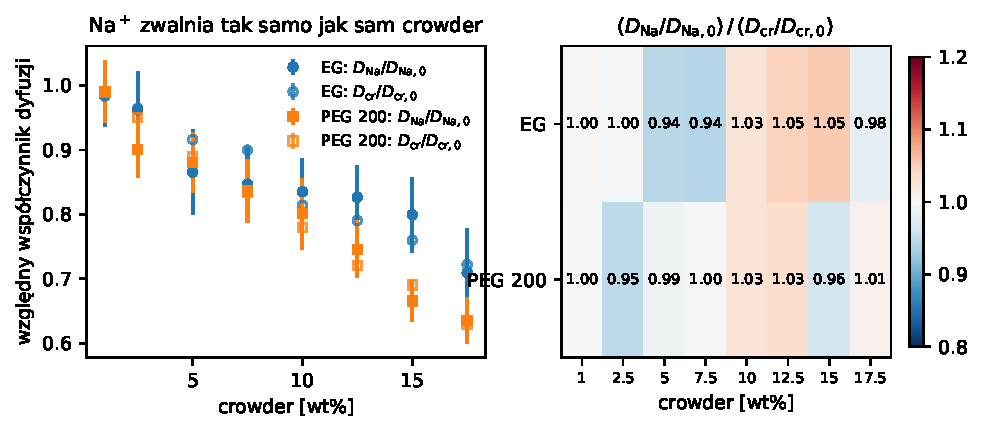
\includegraphics[width=0.85\linewidth]{../knowles_reframe/figures/t1_dosy_ratios.pdf}
\caption{DOSY: w EG i PEG 200 Na$^+$ (pełne symbole) zwalnia dokładnie jak sam crowder (puste). Stosunek $\approx1$ oznacza brak wiązania.}
\end{figure}

Uwaga o wersji z manuskryptu: z poprawką nanolepkości (Tabela S5) wychodzi $\beta n_\text{EG}=\NbnCodeEG\pm\NbnCodeEGErr$~M$^{-1}$. Nawet ta wartość nie ratuje rachunku (sekcja 3).

\section{Skoro nie wiążą, dlaczego destabilizują?}

EG przy 40 wt\% obniża $K$ o $\dG_\text{obs}=+\NddGEGforty$~kJ/mol. To największy efekt w całym zbiorze danych. Zgodnie z naszym rozumowaniem:
\begin{itemize}
\item deplecja jest tu prawie zerowa, a gdyby była, \emph{stabilizowałaby} dupleks;
\item wiązania Na$^+$ nie widać, więc $\dG_\text{el}\approx0$;
\item reszta $\dG_\text{obs}-\dG_\text{el}\approx+15$~kJ/mol jest \emph{dodatnia}, a więc nie może być deplecją.
\end{itemize}
Rysunek 2 pokazuje to wprost. Policzyłem, o ile osłabiłby dupleks ubytek wolnego Na$^+$, gdyby EG wiązał go tyle, ile pozwala DOSY. Nawet przy górnej granicy (zielone pasmo) albo przy wartości z manuskryptu (niebieska linia) to najwyżej $\NegExplCode$~kJ/mol z $\NddGEGforty$, czyli $\NegExplFracCode$\%. Żeby wyjaśnić całość, związane musiałoby być $\NreqFullManFrac$--$\NreqFullConsFrac$\% Na$^+$, a elektroda pokazałaby wtedy $\NreqFullManmV$--$\NreqFullConsmV$~mV; pokazuje około 6~mV.

\begin{figure}[h]
\centering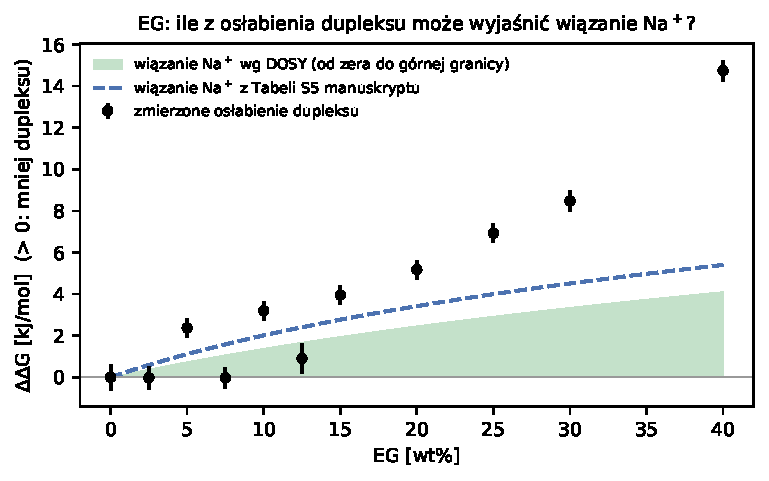
\includegraphics[width=0.62\linewidth]{../knowles_reframe/figures/t1_salt_vs_obs.pdf}
\caption{EG: zmierzone osłabienie dupleksu (punkty) i to, ile mogłoby z niego wynikać z wiązania Na$^+$ (pasmo i linia). Różnica między nimi to efekt, którego wiązanie Na$^+$ nie tłumaczy.}
\end{figure}

To samo dotyczy PEG 200 ($\NNPtwoHobs$~kJ/mol przy 40 wt\%, DOSY: brak wiązania). Wniosek: \textbf{istnieje trzeci, niejonowy człon, który destabilizuje dupleks}. W obecnym rachunku dla długich PEG ten sam człon wpada do „reszty” i zaniża deplecję. Warunek 1 z sekcji 1 nie jest więc spełniony.

\section{Co wiadomo o PEG i soli: PEG sól wypycha}

Pomiary termodynamiczne mierzą, jak PEG zmienia \emph{aktywność} soli, czyli wielkość, którą „czuje” DNA. Konwencja: $\mu_x=\partial\mu_\text{sól}/\partial m_\text{EO}$ na molal grup EO; $\mu_x>0$ oznacza, że sól jest wypychana z otoczenia PEG, a jej aktywność rośnie.

\begin{center}\small
\begin{tabular}{>{\raggedright\arraybackslash}p{5.2cm}>{\raggedright\arraybackslash}p{3.6cm}>{\raggedright\arraybackslash}p{6.2cm}}
\toprule
pomiar & układ & wynik (cal\,mol$^{-1}$molal$^{-1}$ EO)\\
\midrule
VPO, Knowles 2011 & PEG 1000/2000 + KCl & $+32$ do $+38$ (wypychanie)\\
VPO, Knowles 2015, rozkład na jony & grupa EO + jony & Na$^+$ $+4.7\pm2$; Cl$^-$ $+38$; HPO$_4^{2-}$ $+234$\\
\quad z tego dla soli & NaCl; Na$_2$HPO$_4$ (nasz bufor) & $+42\pm3$; $+243\pm7$\\
dyfuzja wieloskładnikowa, Annunziata & PEG 20k + NaCl & $+47$ do $+50$ (2.4 H$_2$O/EO bez soli)\\
dyfuzja, tyloxapol & Na$_2$SO$_4$ & $\approx+190$ (7--8 H$_2$O/EO bez soli)\\
\bottomrule
\end{tabular}
\end{center}

Dwie niezależne metody (osmometria i dyfuzja) zgadzają się dla NaCl z dokładnością do około 15\%. Kolejność anionów jest zawsze ta sama: fosforan, siarczan $\gg$ Cl$^-$ $>$ I$^-$ $>$ SCN$^-$, ClO$_4^-$. Dwa ostatnie mają $\mu_x<0$, czyli wiążą się z PEG. Na$^+$ wychodzi netto bliski zera, z lekkim wypychaniem.

Ten sam znak tłumaczy zjawiska, które nie mają nic wspólnego z DNA:
\begin{itemize}
\item \textbf{osmolalność} PEG + sól jest większa niż suma składników [1--3];
\item \textbf{zamarzanie}: NaCl, NaF obniżają temperaturę krzepnięcia roztworu PEG bardziej niż addytywnie, NaSCN prawie addytywnie [4,5];
\item \textbf{punkt zmętnienia} PEG spada liniowo z molalnością soli, a nachylenie zależy od anionu [6--8];
\item \textbf{układy dwufazowe} PEG--fosforan, PEG--siarczan (z NaCl rozdziału nie ma) [9--11];
\item \textbf{wytrącanie soli przez PEG}, stosowane technologicznie do otrzymywania Na$_2$SO$_4$ i Na$_2$CO$_3$ [12,13];
\item \textbf{dyfuzjoforeza}: PEG wędruje z miejsc o wysokim stężeniu soli do niskiego; zamiana Na$^+$ na K$^+$ prawie nic nie zmienia [14].
\end{itemize}
Przeciwny obraz (PEG wiąże kation) pojawia się w literaturze tylko w nanoporach przy 1--4~M soli [20].

\textbf{Co to znaczy dla $K$.} Dupleks potrzebuje soli: $d\ln K=S_K\,d\ln a_\pm$. Skoro PEG podnosi aktywność soli, kanał solny \emph{stabilizuje} dupleks: $\Delta\ln K\approx+0.3$ (jak NaCl) do $+1.2$ (jak Na$_2$HPO$_4$) przy 10 wt\% długiego PEG. Kierunek jest odwrotny do założenia manuskryptu.

\section{Co to znaczy mikroskopowo i jak to pogodzić z naszym DOSY}

\textbf{Obraz mikroskopowy.} Każda grupa EO wiąże wiązaniami wodorowymi kilka cząsteczek wody (tlen eterowy jest akceptorem). Jony też mają własne, silnie związane otoczki hydratacyjne. Żeby jon wszedł w otoczkę PEG, musiałby się z nią „podzielić” wodą, co jest niekorzystne, zwłaszcza dla silnie hydratowanych anionów (fosforan, siarczan). Wokół łańcucha powstaje więc warstwa wody uboższa w sól. Wypychanie soli oznacza więc, że część wody jest dla soli niedostępna. Sól mieści się w mniejszej objętości „wolnej” wody, więc jej efektywne stężenie i aktywność rosną. Do opisu wystarcza jedna liczba: $n_w$, czyli ile cząsteczek wody na grupę EO jest „zajętych” dla soli.

\textbf{Gdzie w tym obrazie jest DOSY.} Na$^+$ może też chwilowo koordynować tlen eterowy (słabo; nawet 18-korona-6 wiąże Na$^+$ w wodzie z $\log K\approx0.8$). Te krótkie kontakty to dokładnie to, co widzi DOSY w długich PEG: Na$^+$, który przez ułamek czasu porusza się razem z łańcuchem, dyfunduje wolniej. Oba efekty mogą istnieć \emph{jednocześnie}. Liczy się bilans:
\[
\mu_+\;=\;RT\Big(\underbrace{\tfrac{n_w}{55.5}}_{\text{wypychanie z otoczki}}\;-\;\underbrace{\kappa}_{\text{kontakty (DOSY)}}\Big).
\]
DOSY mierzy tylko drugi człon: kontakty spowalniają jon, a jon wypchnięty z otoczki dyfunduje w objętości jak zwykle. VPO i aktywność widzą sumę. Przy VPO $\mu_+(\text{Na}^+)=+4.7$~cal oba człony muszą się prawie znosić. Wymaga to $n_w=\NNnwLo$ cząsteczek wody na EO dla $\kappa=0.055$ albo $n_w=\NNnwHi$ dla $\kappa=0.168$~M$^{-1}$. Dla porównania dyfuzjoforeza daje 2.4~H$_2$O/EO w NaCl i 7.7 w Na$_2$SO$_4$. Niższy wariant DOSY jest więc w pełni zgodny z VPO, a wyższy leży na granicy.

\textbf{Elektroobojętność.} Na$^+$ nie może oddalić się od swojego anionu. Fosforan, który dominuje w naszym buforze, jest wypychany najsilniej ze wszystkich jonów ($+234$). Ciągnie więc Na$^+$ za sobą, a dla DNA liczy się aktywność soli jako całości, $a_\pm$, a nie samego Na$^+$.

\begin{figure}[h]
\centering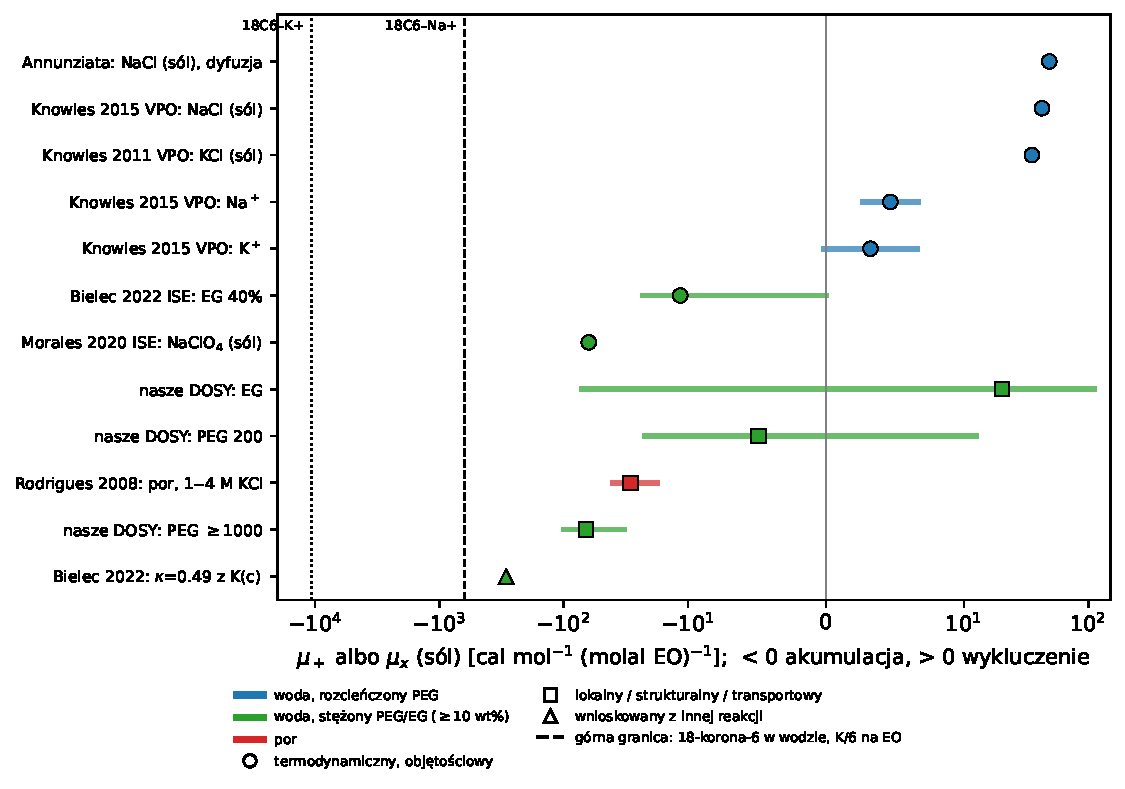
\includegraphics[width=0.9\linewidth]{q8_cation_binding.pdf}
\caption{Wszystkie dane o „wiązaniu” kationu przez PEG na jednej osi. Pomiary termodynamiczne w rozcieńczonej wodzie (niebieskie) dają wypychanie soli albo zero dla Na$^+$. Ujemne (akumulacja) są tylko pomiary lokalne lub transportowe (kwadraty, w tym nasze DOSY) oraz wartość wywnioskowana z $K(c)$ w Bielec 2022 (trójkąt).}
\end{figure}

\begin{wniosek}
DOSY i VPO sobie nie przeczą. DOSY pokazuje realne, krótkie kontakty Na$^+$ z łańcuchem. Nie mierzy jednak aktywności soli, a to ona wchodzi do $K$. W bilansie termodynamicznym kontakty są skompensowane wypychaniem z otoczki, a sól jako całość jest wypychana.
\end{wniosek}

\section{Interpretacja Knowlesa}

Knowles i in. (PNAS 2011, grupa Recorda) zmierzyli to samo zjawisko na dupleksie 12 bp: EG i krótkie PEG destabilizują, długie stabilizują, a przy około 6 molal monomeru stabilizacja się odwraca. Rozkładają efekt na molal monomeru PEG ($m_3$) na trzy człony:
\[
\frac{\partial\Delta G^\circ}{\partial m_3}=\underbrace{\Delta\mu^\text{pi}}_{\text{oddz. z zasadami}}+\underbrace{\Delta\mu^\text{ev}}_{\text{obj. wyłączona}}+\underbrace{\text{poprawka solna}}_{\mu_{x}>0\text{ z VPO}}.
\]
\begin{itemize}
\item \textbf{Oddziaływania z zasadami.} Glikol nieco woli otaczać aromatyczne powierzchnie zasad, które odsłaniają się przy rozpleceniu dupleksu. Człon jest proporcjonalny do odsłanianej powierzchni, więc sprzyja stanowi rozplecionemu. To jest brakujący „trzeci człon” z sekcji 3. Wymagana energia jest mała: około 1\% zmiany rozpuszczalności zasady na molal EG.
\item \textbf{Objętość wyłączona} (Hermans) stabilizuje dupleks; na monomer jest stała dla długich PEG.
\item \textbf{Ułamek segmentów dostępnych dla DNA} ($\chi$): 1 dla EG, około 0.5 dla długich PEG, bo środek kłębka jest schowany. W splątanej sieci (około 6 monomolal) DNA znów „widzi” wszystkie segmenty ($\chi\to1$), więc destabilizacja wraca. Tak powstaje odwrócenie.
\item \textbf{Sól} wchodzi tylko przez aktywność (VPO) i daje mały, \emph{stabilizujący} wkład.
\end{itemize}

\textbf{Liczby Knowlesa przeniesione na nasz układ bez dopasowania} odtwarzają EG 40\% ($\LegKnowlesfourzero$ vs zmierzone $\LegObsfourzero$~kJ/mol), PEG 200 40\% ($\LpegTwoKnowlesfourzero$ vs $\LpegTwoObsfourzero$) i długie PEG przy 20--40 wt\% (rys.~\ref{fig:budget}). Nie odtwarzają tylko szybkiego początku stabilizacji przy kilku wt\%.

\begin{figure}[h]
\centering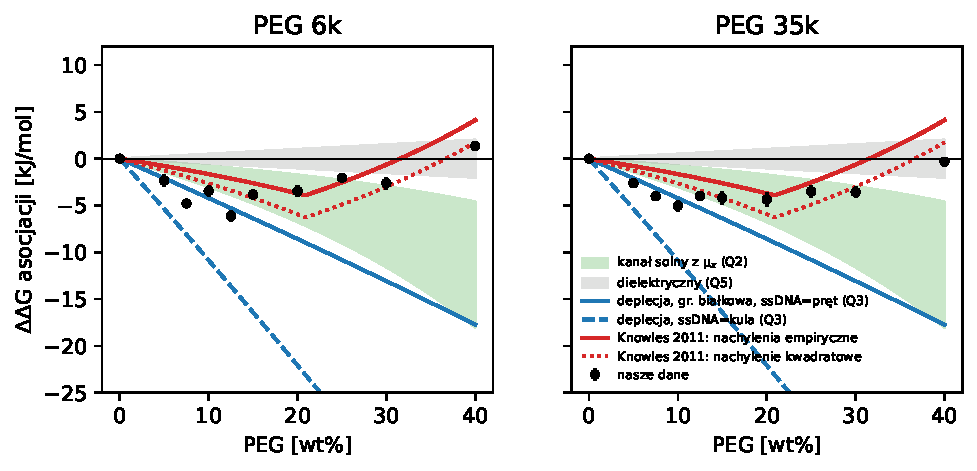
\includegraphics[width=0.95\linewidth]{lit_budget.pdf}
\caption{Nasze dane (punkty) i przewidywanie z liczb Knowlesa bez dopasowania (czerwone). Szare i zielone pasma: kanał solny i efekt dielektryczny z literatury.}
\label{fig:budget}
\end{figure}

\textbf{Niezależne sprawdzenie: model najbliższych sąsiadów w zatłoczeniu} (Ghosh, \dots, Sugimoto, PNAS 2020). Grupa Sugimoto wyznaczyła parametry nearest-neighbour w 40 wt\% PEG 200 i rozszerzyła je na inne kosoluty: $\Delta G_\text{NN}=\Delta G_\text{NN,sól}+m_\text{cs}\,\Delta a_w$. Interpretują to przez aktywność wody, ale sami dostają \emph{trzy różne} nachylenia dla trzech klas kosolutów (PEG; EG/glicerol; 1,3-propanodiol/2-metoksyetanol). To jest właśnie chemiczna specyficzność, którą opisuje Knowles. Objętość wyłączoną dla dużych PEG dodają osobno (Hermans), a efekt PEG 200 jest u nich ten sam w 0.1 i 1~M NaCl, więc jony w nim nie grają roli. Dla naszej sekwencji suma $m_\text{cs}$ wynosi $\NNmPEG$ (klasa PEG) i $\NNmEG$ (klasa EG)~kcal/mol na jednostkę $\Delta a_w$. Przewidywanie bez żadnego dopasowania, 40 wt\%, kJ/mol:

\begin{center}\small
\begin{tabular}{lcccc}
\toprule
crowder & zmierzone & NN, $a_w$ z modelu & NN, $a_w$ z VPO (Nakano 2004) & reszta = zmierzone $-$ NN\\
\midrule
EG & $\NNEGobs$ & $\NNEGpred$ & $\NNEGnak$ & $\NNEGres$\\
PEG 200 & $\NNPtwoHobs$ & $\NNPtwoHpred$ & $\NNPtwoHnak$ & $\NNPtwoHres$\\
PEG 1000 & $\NNPonekobs$ & $\NNPonekpred$ & $\NNPoneknak$ & $\NNPonekres$\\
PEG 6000 & $\NNPsixkobs$ & $\NNPsixkpred$ & -- & $\NNPsixkres$\\
PEG 35000 & $\NNPthirtyfivekobs$ & $\NNPthirtyfivekpred$ & -- & $\NNPthirtyfivekres$\\
\bottomrule
\end{tabular}
\end{center}
EG wychodzi ilościowo. Dla długich PEG reszta jest ujemna i dla PEG $\geq$3000 przy 10--40 wt\% mieści się w przedziale od $\NNresLo$ do $\NNresHi$~kJ/mol. Taka powinna być deplecja. Zastrzeżenia: parametry wyznaczono przy 37~°C i 100~mM NaCl, a $a_w$ długich PEG jest niepewne około trzykrotnie (\texttt{q9\_nn\_sugimoto.py}). Klasyczny NN (SantaLucia) daje dla naszego dupleksu w buforze $K_0\approx\NNKsl\cdot10^9$~M$^{-1}$ wobec zmierzonego $\NNKobs\cdot10^9$, czyli różnicę $\NNdGdiff$~kJ/mol, w granicach typowej dokładności NN przy niskiej soli.

\begin{wniosek}
Trzy niezależne opisy, Knowlesa, Sugimoto i nasz pomiar DOSY dla EG, prowadzą do tego samego wniosku. Destabilizację daje niejonowy człon chemiczny, stabilizację objętość wyłączona, a odwrócenie wynika z ich różnej zależności od stężenia. Do opisu $K$ wiązanie Na$^+$ nie jest potrzebne.
\end{wniosek}

\section{Jak można ująć nasz artykuł}

\textbf{Co zostaje bez zmian.} Dane $K$ dla EG i PEG 200--35k (szeroki zakres $M$, niska sól, FCS-FRET), pomiary DOSY oraz pomysł z sekcji 1: deplecja jako reszta i jej skalowanie $V_\text{eff}/(R_g\,\xi\,R_g^\text{ssDNA})$ (Fig.~4f).

\textbf{Co się zmienia.} Od $\dG_\text{obs}$ odejmujemy człon chemiczny i solny wyznaczony \emph{niezależnie}, bez dopasowania do naszych danych:
\[
\dG_\text{depl}=\dG_\text{obs}-\underbrace{\dG_\text{chem}}_{\text{Knowles / NN-Sugimoto}}-\underbrace{\dG_\text{sól}}_{\text{VPO, mały, }<0}.
\]
Wtedy oba warunki z sekcji 1 są spełnione: dla EG i PEG 200 reszta wynosi około zera, a dla długich PEG jest ujemna i prawie stała.

\textbf{Możliwa oś artykułu:}
\begin{enumerate}
\item \textbf{Ilościowy rozkład efektu zatłoczenia na trzy człony} w zakresie $M$ od 62 do 35\,000 g/mol, przy soli 4$\times$ niższej niż u Knowlesa i innej metodzie. Zgodność bez dopasowania z dwiema niezależnymi ramami (Knowles, Sugimoto) jest mocnym argumentem za jakością naszych $K$.
\item \textbf{Deplecja wyznaczona jako reszta} po odjęciu niezależnie znanego członu chemicznego. To nasz nowy wkład: $V_\text{eff}$ ze skalowaniem z $\xi$, czego Knowles nie miał.
\item \textbf{PEG--Na$^+$: kontakty istnieją, ale nie sterują $K$.} DOSY pokazuje krótkie kontakty Na$^+$ z długimi PEG. Bilans z literaturą (VPO, dyfuzjoforeza) pokazuje, że kompensuje je wypychanie soli z otoczki, a dla EG i PEG 200 kontaktów nie ma wcale. To porządkuje też wynik Bielec 2022.
\end{enumerate}

\textbf{Czego \emph{nie} możemy twierdzić:} że odwrócenie stabilizacji jest nowe (opisał je Knowles 2011, Fig.~4) ani że wynika z sekwestracji Na$^+$.

\textbf{Co rozstrzygnęłoby resztę wątpliwości (opcjonalnie):}
\begin{itemize}
\item VPO lub osmometria dla PEG + NaPi w naszym buforze, czyli bezpośredni pomiar $\mu_x$ (oczekiwany sygnał 36--205 mOsm przy precyzji 1--2 mOsm);
\item $K$ w funkcji Na$^+$ przez maksimum (około 150~mM) w buforze, EG i PEG 35k. Wiązanie Na$^+$ przesuwa maksimum w prawo, wypychanie soli w lewo, a efekt niejonowy go nie przesuwa.
\end{itemize}

\vspace{1em}
\hrule
\subsection*{Źródła do sekcji 4}
\footnotesize
\begin{enumerate}[label={[\arabic*]},leftmargin=*,itemsep=0pt]
\item Michel B.E. \emph{Plant Physiol.} 72, 66 (1983). DOI 10.1104/pp.72.1.66
\item Knowles D.B. et al. \emph{PNAS} 108, 12699 (2011). DOI 10.1073/pnas.1103382108
\item Knowles D.B. et al. \emph{Biochemistry} 54, 3528 (2015). DOI 10.1021/acs.biochem.5b00246
\item Sørensen I.E., Thormann E. \emph{Langmuir} 42, 6261 (2026). DOI 10.1021/acs.langmuir.5c05841
\item Gosh R.C., Toda A., Tanaka S. \emph{Polymer} 50, 1304 (2009). DOI 10.1016/j.polymer.2008.12.044
\item Bailey F.E., Callard R.W. \emph{J. Appl. Polym. Sci.} 1, 56 (1959). DOI 10.1002/app.1959.070010110
\item Florin E., Kjellander R., Eriksson J.C. \emph{J. Chem. Soc. Faraday Trans. 1} 80, 2889 (1984). DOI 10.1039/F19848002889
\item Madeira P.P., Uversky V.N., Zaslavsky B.Y. \emph{Int. J. Mol. Sci.} 26, 4545 (2025). DOI 10.3390/ijms26104545
\item da Silva L.H.M., Loh W. \emph{J. Phys. Chem. B} 104, 10069 (2000). DOI 10.1021/jp000719t
\item Bonnassieux S. et al. \emph{Faraday Discuss.} 253, 181 (2024). DOI 10.1039/D4FD00058G
\item Huddleston J.G., Willauer H.D., Rogers R.D. \emph{J. Chem. Eng. Data} 48, 1230 (2003). DOI 10.1021/je034042p
\item Taboada M.E. et al. \emph{J. Chromatogr. B} 743, 101 (2000). DOI 10.1016/S0378-4347(00)00110-9
\item Taboada M.E., Graber T.A., Cisternas L.A. \emph{Ind. Eng. Chem. Res.} 43, 835 (2004). DOI 10.1021/ie030692a
\item Annunziata O. \emph{Molecules} 29, 1367 (2024). DOI 10.3390/molecules29061367
\setcounter{enumi}{19}
\item Breton M.F. et al. \emph{J. Phys. Chem. Lett.} 4, 2202 (2013). DOI 10.1021/jz400938q
\end{enumerate}
\subsection*{Pozostałe}
Ghosh S. et al. \emph{PNAS} 117, 14194 (2020), DOI 10.1073/pnas.1920886117; Ghosh S. et al. \emph{NAR} 47, 3284 (2019), DOI 10.1093/nar/gkz071; Nakano S. et al. \emph{JACS} 126, 14330 (2004), DOI 10.1021/ja0463029; SantaLucia J. \emph{PNAS} 95, 1460 (1998), DOI 10.1073/pnas.95.4.1460; Bielec K. et al. \emph{J. Phys. Chem. Lett.} 13, 112 (2022), DOI 10.1021/acs.jpclett.1c03596. Pełna lista i notatki: \texttt{salt\_exclusion/notes.md}, \texttt{salt\_shift/report.pdf}, \texttt{../knowles\_reframe/report.pdf}.
\normalsize
\end{document}
